%================================================
%   柏原正樹
%   超函数の構造について
%================================================

% -----------------------
% preamble
% -----------------------
% ここから本文 (\begin{document}) までの
% ソースコードに変更を加えた場合は
% 編集者まで連絡してください. 
% Don't change preamble code yourself. 
% If you add something
% (usepackage, newtheorem, newcommand, renewcommand),
% please tell it 
% to the editor of institutional paper of RUMS.

% ------------------------
% documentclass
% ------------------------
\documentclass[9pt, b5paper, dvipdfmx, leqno]{jsarticle}

% ------------------------
% usepackage
% ------------------------
\usepackage{algorithm}
\usepackage{algorithmic}
\usepackage{amscd}
\usepackage{amsfonts}
\usepackage{amsmath}
\usepackage[psamsfonts]{amssymb}
\usepackage{amsthm}
\usepackage{ascmac}
\usepackage{bm}
\usepackage{color}
\usepackage{enumerate}
\usepackage{fancybox}
\usepackage[stable]{footmisc}
\usepackage{graphicx}
\usepackage{listings}
\usepackage{mathrsfs}
\usepackage{mathtools}
\usepackage{otf}
\usepackage{pifont}
\usepackage{proof}
\usepackage{subfigure}
\usepackage{tikz}
\usepackage{verbatim}
\usepackage[all]{xy}
\usepackage{url}
\usetikzlibrary{cd}



% ================================
% パッケージを追加する場合のスペース 
%\usepackage{calligra}
\usepackage[dvipdfmx]{hyperref}
\usepackage{xcolor}
\definecolor{darkgreen}{rgb}{0,0.45,0} 
\definecolor{darkred}{rgb}{0.75,0,0}
\definecolor{darkblue}{rgb}{0,0,0.6} 
\hypersetup{
    colorlinks=true,
    citecolor=darkgreen,
    linkcolor=darkred,
    urlcolor=darkblue,
}
\usepackage{pxjahyper}
\usepackage{layout}
\usepackage{caption}

%=================================


% =================================


% ----------------------------
% commmand
% ----------------------------
% 執筆に便利なコマンド集です. 
% コマンドを追加する場合は下のスペースへ. 

% 集合の記号 (黒板文字)
\newcommand{\NN}{\mathbb{N}}
\newcommand{\ZZ}{\mathbb{Z}}
\newcommand{\QQ}{\mathbb{Q}}
\newcommand{\RR}{\mathbb{R}}
\newcommand{\CC}{\mathbb{C}}
\newcommand{\PP}{\mathbb{P}}
\newcommand{\KK}{\mathbb{K}}


% 集合の記号 (太文字)
\newcommand{\nn}{\mathbf{N}}
\newcommand{\zz}{\mathbf{Z}}
\newcommand{\qq}{\mathbf{Q}}
\newcommand{\rr}{\mathbf{R}}
\newcommand{\cc}{\mathbf{C}}
\newcommand{\pp}{\mathbf{P}}
\newcommand{\kk}{\mathbf{K}}

% 特殊な写像の記号
\newcommand{\ev}{\mathop{\mathrm{ev}}\nolimits} % 値写像
\newcommand{\pr}{\mathop{\mathrm{pr}}\nolimits} % 射影

% スクリプト体にするコマンド
%   例えば {\mcal C} のように用いる
\newcommand{\mcal}{\mathcal}

% 花文字にするコマンド 
%   例えば {\h C} のように用いる
\newcommand{\h}{\mathscr}

% ヒルベルト空間などの記号
\newcommand{\F}{\mcal{F}}
\newcommand{\X}{\mcal{X}}
\newcommand{\Y}{\mcal{Y}}
\newcommand{\Hil}{\mcal{H}}
\newcommand{\RKHS}{\Hil_{k}}
\newcommand{\Loss}{\mcal{L}_{D}}
\newcommand{\MLsp}{(\X, \Y, D, \Hil, \Loss)}

% 偏微分作用素の記号
\newcommand{\p}{\partial}

% 角カッコの記号 (内積は下にマクロがあります)
\newcommand{\lan}{\langle}
\newcommand{\ran}{\rangle}



% 圏の記号など
\newcommand{\Set}{{\bf Set}}
\newcommand{\Vect}{{\bf Vect}}
\newcommand{\FDVect}{{\bf FDVect}}
\newcommand{\Mod}{\mathop{\mathrm{Mod}}\nolimits}
\newcommand{\CGA}{{\bf CGA}}
\newcommand{\GVect}{{\bf GVect}}
\newcommand{\Lie}{{\bf Lie}}
\newcommand{\dLie}{{\bf Liec}}



% 射の集合など
\newcommand{\Map}{\mathop{\mathrm{Map}}\nolimits}
\newcommand{\Hom}{\mathop{\mathrm{Hom}}\nolimits}
\newcommand{\End}{\mathop{\mathrm{End}}\nolimits}
\newcommand{\Aut}{\mathop{\mathrm{Aut}}\nolimits}
\newcommand{\Mor}{\mathop{\mathrm{Mor}}\nolimits}

% その他便利なコマンド
\newcommand{\dip}{\displaystyle} % 本文中で数式モード
\newcommand{\e}{\varepsilon} % イプシロン
\newcommand{\dl}{\delta} % デルタ
\newcommand{\pphi}{\varphi} % ファイ
\newcommand{\ti}{\tilde} % チルダ
\newcommand{\pal}{\parallel} % 平行
\newcommand{\op}{{\rm op}} % 双対を取る記号
\newcommand{\lcm}{\mathop{\mathrm{lcm}}\nolimits} % 最小公倍数の記号
\newcommand{\Probsp}{(\Omega, \F, \P)} 
\newcommand{\argmax}{\mathop{\rm arg~max}\limits}
\newcommand{\argmin}{\mathop{\rm arg~min}\limits}





% ================================
% コマンドを追加する場合のスペース 
\renewcommand\proofname{\bf 証明} % 証明
\numberwithin{equation}{subsection}
\newcommand{\cTop}{\textsf{Top}}
%\newcommand{\cOpen}{\textsf{Open}}
\newcommand{\Op}{\mathop{\textsf{Open}}\nolimits}
\newcommand{\Ob}{\mathop{\textrm{Ob}}\nolimits}
\newcommand{\id}{\mathop{\mathrm{id}}\nolimits}
\newcommand{\pt}{\mathop{\mathrm{pt}}\nolimits}
\newcommand{\res}{\mathop{\rho}\nolimits}
\newcommand{\Ring}{\mathop{\textsf{Ring}}\nolimits}
\newcommand{\cAb}{\mathop{\textsf{Ab}}\nolimits}
\newcommand{\Sh}{\mathop{\textsf{Sh}}\nolimits}
\newcommand{\PSh}{\mathop{\textsf{PSh}}\nolimits}
\newcommand{\Ker}{\mathop{\mathrm{Ker}}\nolimits}
\newcommand{\im}{\mathop{\mathrm{Im}}\nolimits}
\newcommand{\Coker}{\mathop{\mathrm{Coker}}\nolimits}
\newcommand{\Coim}{\mathop{\mathrm{Coim}}\nolimits}
\newcommand{\Ht}{\mathop{\mathrm{Ht}}\nolimits}
\newcommand{\colim}{\mathop{\mathrm{colim}}}
\newcommand{\ori}{\mathop{\textsf{or}}\nolimits}


\newcommand{\cat}{\mathcal{C}}%一般の圏の記号
\newcommand{\Comp}{\mathop{\mathrm{C}}\nolimits}%複体の圏
\newcommand{\Komp}{\mathop{\mathrm{K}}\nolimits}%複体のホモトピー圏
\newcommand{\CCat}{\Comp(\cat)}%圏Cの複体の圏
\newcommand{\KCat}{\Komp(\cat)}%圏Cの複体のホモトピー圏
\newcommand{\HOM}{\mathop{\mathscr{H}\hspace{-2pt}om}\nolimits}%内部Hom
\newcommand{\RHOM}{\mathop{\mathrm{R}\hspace{-1.5pt}\HOM}\nolimits}
\newcommand{\muS}{\mathop{\mathrm{SS}}\nolimits}
\newcommand{\RG}{\mathop{\mathrm{R}\hspace{-0pt}\Gamma}\nolimits}

\newcommand{\limf}{\mathop{\text{``}\hspace{-0.7pt}\varinjlim\hspace{-1.5pt}\text{''}}}
\newcommand{\sumf}{\mathop{\text{``}\hspace{-0.7pt}\bigoplus\hspace{-1.5pt}\text{''}}}

\newcommand{\hh}{\mathop{\mathrm{h}}\nolimits}
\newcommand{\Ind}{\mathop{\mathrm{Ind}}}


%筆記体
\newcommand{\cA}{\mcal{A}}
\newcommand{\cB}{\mcal{B}}
\newcommand{\cC}{\mcal{C}}
\newcommand{\cD}{\mcal{D}}
\newcommand{\cE}{\mcal{E}}
\newcommand{\cF}{\mcal{F}}
\newcommand{\cG}{\mcal{G}}
\newcommand{\cH}{\mcal{H}}
\newcommand{\cI}{\mcal{I}}
\newcommand{\cJ}{\mcal{J}}
\newcommand{\cK}{\mcal{K}}
\newcommand{\cL}{\mcal{L}}
\newcommand{\cM}{\mcal{M}}
\newcommand{\cN}{\mcal{N}}
\newcommand{\cO}{\mcal{O}}
\newcommand{\cP}{\mcal{P}}
\newcommand{\cQ}{\mcal{Q}}
\newcommand{\cR}{\mcal{R}}
\newcommand{\cS}{\mcal{S}}
\newcommand{\cT}{\mcal{T}}
\newcommand{\cU}{\mcal{U}}
\newcommand{\cV}{\mcal{V}}
\newcommand{\cW}{\mcal{W}}
\newcommand{\cX}{\mcal{X}}
\newcommand{\cY}{\mcal{Y}}
\newcommand{\cZ}{\mcal{Z}}

%スクリプト体
\newcommand{\scA}{\mathscr{A}}
\newcommand{\scB}{\mathscr{B}}
\newcommand{\scC}{\mathscr{C}}
\newcommand{\scD}{\mathscr{D}}
\newcommand{\scE}{\mathscr{E}}
\newcommand{\scF}{\mathscr{F}}
\newcommand{\scG}{\mathscr{G}}
\newcommand{\scH}{\mathscr{H}}
\newcommand{\scI}{\mathscr{I}}
\newcommand{\scJ}{\mathscr{J}}
\newcommand{\scK}{\mathscr{K}}
\newcommand{\scL}{\mathscr{L}}
\newcommand{\scM}{\mathscr{M}}
\newcommand{\scN}{\mathscr{N}}
\newcommand{\scO}{\mathscr{O}}
\newcommand{\scP}{\mathscr{P}}
\newcommand{\scQ}{\mathscr{Q}}
\newcommand{\scR}{\mathscr{R}}
\newcommand{\scS}{\mathscr{S}}
\newcommand{\scT}{\mathscr{T}}
\newcommand{\scU}{\mathscr{U}}
\newcommand{\scV}{\mathscr{V}}
\newcommand{\scW}{\mathscr{W}}
\newcommand{\scX}{\mathscr{X}}
\newcommand{\scY}{\mathscr{Y}}
\newcommand{\scZ}{\mathscr{Z}}


\newcommand{\ibA}{\mathop{\text{\textit{\textbf{A}}}}}
\newcommand{\ibB}{\mathop{\text{\textit{\textbf{B}}}}}
\newcommand{\ibC}{\mathop{\text{\textit{\textbf{C}}}}}
\newcommand{\ibD}{\mathop{\text{\textit{\textbf{D}}}}}
\newcommand{\ibE}{\mathop{\text{\textit{\textbf{E}}}}}
\newcommand{\ibF}{\mathop{\text{\textit{\textbf{F}}}}}
\newcommand{\ibG}{\mathop{\text{\textit{\textbf{G}}}}}
\newcommand{\ibH}{\mathop{\text{\textit{\textbf{H}}}}}
\newcommand{\ibI}{\mathop{\text{\textit{\textbf{I}}}}}
\newcommand{\ibJ}{\mathop{\text{\textit{\textbf{J}}}}}
\newcommand{\ibK}{\mathop{\text{\textit{\textbf{K}}}}}
\newcommand{\ibL}{\mathop{\text{\textit{\textbf{L}}}}}
\newcommand{\ibM}{\mathop{\text{\textit{\textbf{M}}}}}
\newcommand{\ibN}{\mathop{\text{\textit{\textbf{N}}}}}
\newcommand{\ibO}{\mathop{\text{\textit{\textbf{O}}}}}
\newcommand{\ibP}{\mathop{\text{\textit{\textbf{P}}}}}
\newcommand{\ibQ}{\mathop{\text{\textit{\textbf{Q}}}}}
\newcommand{\ibR}{\mathop{\text{\textit{\textbf{R}}}}}
\newcommand{\ibS}{\mathop{\text{\textit{\textbf{S}}}}}
\newcommand{\ibT}{\mathop{\text{\textit{\textbf{T}}}}}
\newcommand{\ibU}{\mathop{\text{\textit{\textbf{U}}}}}
\newcommand{\ibV}{\mathop{\text{\textit{\textbf{V}}}}}
\newcommand{\ibW}{\mathop{\text{\textit{\textbf{W}}}}}
\newcommand{\ibX}{\mathop{\text{\textit{\textbf{X}}}}}
\newcommand{\ibY}{\mathop{\text{\textit{\textbf{Y}}}}}
\newcommand{\ibZ}{\mathop{\text{\textit{\textbf{Z}}}}}

\newcommand{\ibx}{\mathop{\text{\textit{\textbf{x}}}}}

\numberwithin{equation}{section}














\newcommand{\hocolim}{{\mathrm{hocolim}}}
\newcommand{\indlim}[1][]{\mathop{\varinjlim}\limits_{#1}}
\newcommand{\sindlim}[1][]{\smash{\mathop{\varinjlim}\limits_{#1}}\,}
\newcommand{\prolim}[1][]{\mathop{\varprojlim}\limits_{#1}}
\newcommand{\sprolim}[1][]{\smash{\mathop{\varprojlim}\limits_{#1}}\,}

\newcommand{\tens}[1][]{\mathbin{\otimes_{\raise1.5ex\hbox to-.1em{}{#1}}}}
\newcommand{\etens}{\mathbin{\boxtimes}}
\newcommand{\ltens}[1][]{\mathbin{\overset{\mathrm{L}}\tens}_{#1}}
\newcommand{\mtens}[1][]{\mathbin{\overset{\mathrm{\mu}}\tens}_{#1}}
\newcommand{\lltens}[1][]{{\mathop{\tens}\limits^{\mathrm{L}}_{#1}}}
\newcommand{\letens}{\overset{\mathrm{L}}{\etens}}
\newcommand{\detens}{\underline{\etens}}
\newcommand{\ldetens}{\overset{\mathrm{L}}{\underline{\etens}}}
\newcommand{\dtens}[1][]{{\overset{\mathrm{L}}{\underline{\otimes}}}_{#1}}

\newcommand{\simar}{\mathrel{\overset{\sim}{\rightarrow}}}%同型右矢印
\newcommand{\simarr}{\mathrel{\overset{\sim}{\longrightarrow}}}%同型右矢印
\newcommand{\simra}{\mathrel{\overset{\sim}{\leftarrow}}}%同型左矢印
\newcommand{\simrra}{\mathrel{\overset{\sim}{\longleftarrow}}}%同型左矢印

% =================================


%================================================
% 自前の定理環境
%   https://mathlandscape.com/latex-amsthm/
% を参考にした
\newtheoremstyle{mystyle}%   % スタイル名
    {5pt}%                   % 上部スペース
    {5pt}%                   % 下部スペース
    {}%              % 本文フォント
    {}%                  % 1行目のインデント量
    {\bfseries}%                      % 見出しフォント
    {.}%                     % 見出し後の句読点
    {12pt}%                     % 見出し後のスペース
    {\thmname{#1}\thmnumber{ #2}\thmnote{{\hspace{2pt}\normalfont (#3)}}}% % 見出しの書式

\theoremstyle{mystyle}
\newtheorem{AXM}{公理}[section]
\newtheorem{DFN}[AXM]{定義}
\newtheorem{THM}[AXM]{定理}
\newtheorem*{THM*}{定理}
\newtheorem{PRP}[AXM]{命題}
\newtheorem{LMM}[AXM]{補題}
\newtheorem{CRL}[AXM]{系}
\newtheorem{EG}[AXM]{例}
\newtheorem{CNV}[AXM]{規約}


% 定理環境ここまで
%====================================================

%レイアウト
%\setlength{\oddsidemargin}{-10pt}
%\setlength{\evensidemargin}{10pt}

% ---------------------------
% new definition macro
% ---------------------------
% 便利なマクロ集です

% 内積のマクロ
%   例えば \inner<\pphi | \psi> のように用いる
\def\inner<#1>{\langle #1 \rangle}

% ================================
% マクロを追加する場合のスペース 
\def\ind<#1>{\mathop{\text{``}\hspace{-0.7pt}#1\limits\hspace{-1.5pt}\text{''}}}

%=================================






% ----------------------------
% documenet 
% ----------------------------
% 以下, 本文の執筆スペースです. 
% Your main code must be written between 
% begin document and end document.
% ---------------------------

\title{超函数の構造について}
\author{柏原正樹\thanks{東大数学教室}}
\date{}
\begin{document}
\maketitle

``この世・現実世界''(実数の世界)と``あの世・ゆうれいの世界''(複素数
領域)の境目に立って眺めることによって,
タチの悪い無限大をとらえ\dots\dots

\rightline{---佐藤幹夫---}

\setcounter{section}{-1}
\section{序}

超函数 (hyperfunction) の概念構成の端緒は,
実の上の函数を正則函数の境界値としてとらえることにあった。
$n$変数超函数\(f(x_1,\dots,x_n)\)は,
\(D_{\pm_1,\dots,\pm_n}
=\left\{\im z_1\gtrless 0,\dots,\im z_n\gtrless 0\right\}\)という
領域で定義された
正則函数\(\varphi_{\pm_1,\dots,\pm_n}(z_1,\dots,z_n)\)の
境界値の和としてあらわされる。即ち,
\[
    f(x_1,\dots,x_n)=
    \sum \varphi_{\pm_1,\dots,\pm_n}\left(
        x_{1}\pm i0,\dots,x_{n}\pm i0
    \right)
\]
ここに,超函数\(
    \varphi_{\pm_1,\dots,\pm_n}\left(x_{1}\pm i0,
    \dots,x_{n}\pm i0\right)
\)は,\(
    \lim\limits_{\varepsilon_{j}\downarrow0}
    \varphi_{\pm_1,\dots,\pm_n}\left(x_{1}\pm i\varepsilon_{1},
    \dots,x_{n}\pm i\varepsilon_{n}\right)
\)ともいうべき ``ideal'' function である。
これは,\(f(x_1,\dots,x_n)\)という超函数が,\(
    \varphi\left(x_1\pm i0,\dots,x_n\pm i0\right)
\)という型の超函数の和にあらわされることを示している。
この\(
    \varphi\left(x_1\pm i0,\dots,x_n\pm i0\right)
\)は,通常の超函数に比して,
より単純な構造を持っているということができよう。
この考えを極限にまで敷衍して得られたのが `` \(\scC\)の理論'' と
いわれるもので,
これを用いて超函数の特異性を極めて明瞭に記述することができる。
20世紀後半に入って、H\"ormander 等々によって展開された偏微分方程式論は,
種々様々の評価を駆使した,
いわば,``不等式による''(或は ``量的'')理論といえるだろう。
それに対して,
\(\scC\)の理論は,``幾何学的''(或は ``質的'')偏微分方程式を
開拓していく強力な道具となるであろう。

`` \(\scC\)の理論'' は,数年前から盛んになりつつあった超函数研究の
機運に力を得て,``超函数論'' の創始者佐藤幹夫先生が1969年に建設された。
この小論は,1970年の4月1日から4日にかけて江之島の片瀬において佐藤先生が
行われた連続講演を骨子にしてまとめたものである。
佐藤先生の平易な中にも深い洞察に満ちた語口を復原できませんでしたが,
できるだけ完全な説明と証明を心懸けました。
尚,\(\scC\)の理論に不可欠な cohomology 理論は,
読者の便宜をはかって一番最後にまわしました。


\clearpage
\section{1変数超函数の特異性の分解}

多変数の場合の理解を容易にするために,
まず一変数の場合をとりあつかう。
\(\scO\)によって正則函数のつくる\(D\)上の sheaf を,\(
    \scA =\cO\rvert_{\rr}
\)によって実解析的函数のつくる\(\rr\)上の sheaf をあらわす。

\(\rr\)の区間\(I\), \(I\)の\(\cc\)における近傍\(D\)をとる。

\captionsetup[figure]{labelformat=empty,labelsep=none}
\begin{figure}[htb]
    \centering
    %\scalebox{0.8}{
        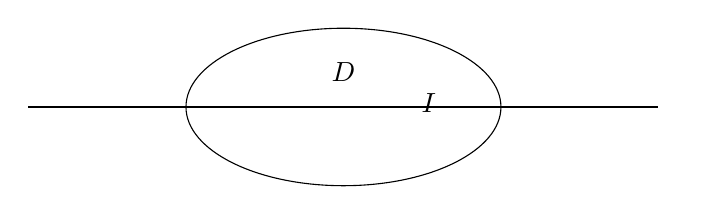
\begin{tikzpicture}[x=1cm]

        \draw[black!100] (0.7,0.1) (0,0) ellipse (2 and 1);
        \draw[,>=stealth,semithick] (-4,0)--(4,0)node[right]{$\rr$}; %x軸
        \draw[thick] (-2,0)--(2,0); %

        \draw (0,0.2) node[above]{$D$};
        \draw (1.3,0.05) node[left]{$I$};
    \end{tikzpicture}%}
     \caption{(1.1)}
    \label{fig:11}
\end{figure}
\setcounter{equation}{1}
\begin{equation}
    \scO(D)\to \scO(D-I)\to\scB(I)\to0    
\end{equation}
という完全列で超函数の層\(\scB\)が定義される。
\(\varphi\in\scO(D-I)\)のあらわす\(I\)上の超函数を\(
    \left[\varphi\right]
\)とかく.

\begin{equation}
    \varepsilon_{\pm}(z)
    =\begin{cases}
        1\ (\im{z}\gtrless0)\\
        0\ (\im{z}\lessgtr0)
    \end{cases}
\end{equation}
によって\(\cc-\rr\)上の函数\(\varepsilon_{\pm}(z)\)を定義すれば,
\(
    g
    =\left[\varphi\right]
    =\left[\varepsilon_{+}\varphi\right]
    -\left[-\varepsilon_{-}\varphi\right]
\)である。
\(
    \varphi\left(x\pm i0\right)
    =\left[\pm\varepsilon_{\pm}\varphi\right]
\)によって超函数\(\varphi\left(x\pm i0\right)\)を定義する。
これらは,正則関数の上半平面(或は下半平面)からの境界値という意味をもつ。
そして
\begin{equation}
    g=
    \left[\varphi\right]
    =\varphi(x+i0)-\varphi(x-i0)\label{eq14}
\end{equation}
は任意の超函数を上半平面からの境界値とか半平面からの境界値との差に
かきあらわす公式である。
\(\scA^{\pm}\)を,
\begin{align*}
    I&\mapsto\indlim \scO\left(D^{\pm}\right)\\
    \text{(但し,}
    &\text{
        \(D\)は\(I\)の近傍を動き,
        \(D^{\pm}=D\cap\cc^{\pm}\)。
    }\\
    &\text{
        \(D^{\pm}=\left\{z\in\cc;\im{z}\gtrless0\right\}\))
    }
\end{align*}
で定義された層とする。

\(\scA^{\pm}\to\scB\)を,\(
    \varphi\in\scA^{\pm}(I)
\)に\(
    \varphi(x\pm i0)\in\scB(I)
\)を対応させる homomorphism とする。
(\(\varphi\)を\(D^{\mp}\)では0に延長することにより,
\(\scO(D-\rr)\)の元とみなす。)
簡単な check によって,これは injective になることがわかる。
従って,\(\scA^{\pm}\)は,正則函数の上半平面(下半平面)からの境界値の
つくる層ということができよう。
\(\varphi\in\scA^{\pm}\)に対して,
\(\varphi(x\pm i0)\in\scA^{\pm}\hookrightarrow\scB\)を
対応させることにより,\(\scA\)の\(\scB\)の中への2つの埋め込み\(
    \scA\to\scA^{+}\to\scB
\)及び\(
    \scA\to\scA^{-}\to\scB
\)が得られる。これは同一になる。
その homomorphism によって実解析函数を超函数と見なす。
一方,式\eqref{eq14}は
\[
    \alpha\colon
    \scA^{+}\oplus\scA^{-}\to\scB
    \quad
    \left(\scA^{+}\ni\varphi,\scA^{-}\ni\psi
    \mapsto
    \varphi(x+i0)+\psi(x-i0)
    \in\scB(I)\right)
\]
が surjective なことをあらわす。
更に\(\scA^{+}\)を\(\scB\)の subsheaf と見做した時,
\(\scA^{+}\cap\scA^{-}=\scA\)。
即ち次の exact sequence が成立つ。
\begin{equation}
    0\to\scA
    \to\scA^{+}\oplus\scA^{-}
    \overset{\alpha}{\to}\scB\to0\label{eq15}
\end{equation}
但し,\(\scA\to\scA^{+}\oplus\scA^{-}\)は,
\(
    \varphi\mapsto
    \left(
        \varphi(x+i0),
        -\varphi(x-i0),
    \right)
\)という homomorphism である。
この完全列は,超関数を,上半平面からの境界値と下半平面からの境界値との差
で書きあらわす方法が\(\scA\)を modulo として
一意的であることをあらわしている。

さて,\eqref{eq15}によって,
\(\alpha\)からただちにみちびかれる sheaf homomorphism \(
    \left(\scA^{+}/\scA\right)\oplus
    \left(\scA^{-}/\scA\right)
    \to\scB/\scA
\)は isomorphism であることがわかる。
これで,\(\scB/\scA\)といういわば超函数の特異性を表現する sheaf を
2つの sheaf の直和により分解することができた。
従って超関数の特異性を,直和因子の各々で眺めてやることによって,
よりくわしく分析することができる。

多変数への拡張を考慮にいれて,上の事実を次の様にいいかえよう。
\(I^{+}\), \(I^{-}\)を\(I\)の2つの copy とする。
\(SI=I^{+}\sqcup I^{-}\), \(\pi\colon SI\to I\)を
その projection とする。
\(I\ni x\)に対して,対応する\(I^{\pm}\)の点を\(x\pm i0\)とかく。
\(x\pm i0\)は,実の点\(x\)に上半平面から近づいたか,
下半平面から近づいたかをあらわす。

%\captionsetup[figure]{labelformat=empty,labelsep=none}
\begin{figure}[htb]
    \centering
    \scalebox{0.8}{
        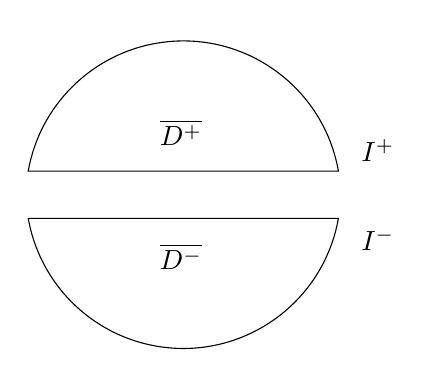
\begin{tikzpicture}[x=1cm]
        \draw (2,0.3)arc(10:170:2)--cycle;
        \draw (2,-0.3)arc(-10:-170:2)--cycle;
        %\draw[black](2,-1)--(2,-1)--(2,-1)arc(0:-180:1)--cycle;

        \draw (0,0.5) node[above]{$\overline{D^+}$};
        \draw (2.5,0.3) node[above]{$I^+$};
        \draw (0,-0.5) node[below]{$\overline{D^-}$};
        \draw (2.5,-0.3) node[below]{$I^-$};
    \end{tikzpicture}}
    \caption{(1.6)}
    \label{fig:16}
\end{figure}

\(I^+\)に\(\scA^{+}\), \(I^-\)に\(\scA^{-}\)の sheaf を
のせることによって\(SI\)上に sheaf \(\widetilde{\scA}\)を定義する。
故に,\(
    \widetilde{\scA}_{x+i0}=\scA^{+}_x
\), \(
    \widetilde{\scA}_{x-i0}=\scA^{-}_x
\)。超函数の特異部分をあらわす sheaf \(\scB/\scA\)を,
\(\widetilde{\scA}\)を使って,
\begin{align*}
    \left(\scB\middle/\scA\right)_x
    &=
    \left(\scA^{+}_x\middle/\scA_x\right)\oplus
    \left(\scA^{-}_x\middle/\scA_x\right)\\
    &=
    \left(\widetilde{\scA}_{x+i0}\middle/\scA_x\right)\oplus
    \left(\widetilde{\scA}_{x-i0}\middle/\scA_x\right)\\
    &=
    \left(\widetilde{\scA}\middle/\pi^{-1}\scA\right)_{x+i0}\oplus
    \left(\widetilde{\scA}\middle/\pi^{-1}\scA\right)_{x-i0}\\
    &=
    \pi_{\ast}\left(\widetilde{\scA}\middle/\pi^{-1}\scA\right)
\end{align*}
と書きあらわすことができる。
\(\scC=\widetilde{\scA}/\pi^{-1}\scA\)と新たに層\(\scC\)を
定義すれば
\begin{equation}
    \scB/\scA=\pi_{\ast}\scC
\end{equation}
これから,
\begin{align*}
    0\to\scA\to\scB\to\pi_{\ast}\scC\to0\\
    0\to\pi^{-1}\scA\to\widetilde{\scA}\to\scC\to0
\end{align*}
の2つの exact sequence が得られる。これは同一になる。
従って,\(\scC\)は超函数の特異性を更にくわしく分解する層というにふさわしい。
以下の章では,これを多変数の場合に一般化する。

\clearpage
\section{Tangential sphere bundle と real monoidal transform}
\(M\)を\(n\)次元実解析的多様体(以下我々がとり扱う category は
実解析的なものばかりであるから,
多様体といえば全て実解析的多様体をあらわす),
\(X\)を\(M\)の複素近傍とする.

\(\scO=\scO_X\)によって,
\(X\)上の holomorphic な函数のつくる\(X\)上の層,
\(\scA=\scA_M=\scO_X\rvert_M\)によって,
実解析函数のつくる\(M\)上の層をあらわす。

\(M\)の tangent vector bundle \(TM\) には,
乗法群\(\rr^+=\{t\in\rr; t>0\}\)が作用している。
\(TM\)から,\(TM\)の zero section \(M\)をひき去った\(
    TM-M
\)を\(\rr^+\)でわって得られた空間を\(SM\)と書く。
\(SM\)は\((n-1)\)次元球面\(S^{n-1}\)を fibre とする\(M\)上の 
sphere bundle である。
\(SM\)を\(M\)の (tangential) sphere bundle とよぶ。
\(M\)の cotangent bundle \(T^{\ast}M\)から
上と同じようにしてつくられた sphere bundle \(
    S^{\ast}M=\left(T^{\ast}M-M\right)/\rr^+
\)を\(M\)の cotangential sphere 
bundle(或は,co-sphere bundle)とよぶ。

解析的には,\(S^{\ast}M\)の方が\(SM\)よりも大きな意味をもっている。
それは,有限階偏微分作用素\(P(x,D)\)に対して\(P_m(x,\eta)\)を
その主要部とすれば,\(P_m(x,D)\)が\(S^{\ast}M\)上の(斉次)函数
となることからも肯ける。
しかし,幾何学的には,むしろ\(SM\)の方が意味をつけやすい。
それは以下の記述で明らかになっていくだろう。

さて,\(X\)の複素構造によって\(X\)の tangent bundle \(TX\)は,
\(TX\rvert_M=TM\oplus\sqrt{-1}TM\)と canonical に分解される。
従って,\(M\)の\(X\)における normal bundle は\(iTM\)と同一視でき,
従って,\(TM\)と同型である。
故に\(M\)の\(X\)における normal sphere 
bundle(normal bundle から zero section を除いた空間
を\(\rr^+\)でわって得られた\(M\)上の sphere bundle)は\(SM\)に
同型である。
\(\tau\colon\widetilde{X}\to X\)を,
\(X\)の\(M\)を中心とする実 monoidal 変換としよう。(\ref{a6}を参照。)
\(\widetilde{X}=\left(X-M\right)SM\)である。
\(x\in M\), \(\xi\in T_xM-\{0\}\)に対して,\(x+i\xi_0\)により
対応する\(SM\)の点をあらわすことにする。
これは,\(x+i\xi_0\in SM\subset\widetilde{X}\)が,
\(i\xi\)という虚の方向から\(x\)に近づいた事を示す適切な表現である\footnote{
    これからわかるように,
    我々が用いる tangential sphere bundle \(SM\)は,
    \(SM\)というより\(iSM\)というべきものである。
}。

\(\omega=\omega_M\)によって,
\(M\)上の orientation bundle をあらわす\footnote{
    以下\(\omega\)を使うのが煩雑と思う方は,
    最初から\(M\)は向きづけられていると仮定して,
    \(\omega\)を無視されてよい。
}。\(\omega\)は局所的には,
\(\zz\)を fibre とする constant sheaf \(\zz_M\)に同型であり,
連結開集合\(U\subset M\)に対して
\[
    \Gamma(U;\omega)\cong
    \begin{cases}
        \zz\quad\text{もしも\(U\)が orientable}\\
        0\quad\text{もしも\(U\)が non orientable}
    \end{cases}
\]が成立つ。
更に,上の\(\Gamma(U;\omega)\cong\zz\)の同型は,
\(U\)の ``向き'' のとり方によって正負の違いがでてくる。
明らかに,\(\omega\tens[\zz_M]\omega=\zz_M\)が成立つ。















\clearpage
\appendix
%\section{実 monoidal 変換について}

\setcounter{section}{5}
\section{実 monoidal 変換について}\label{a6}

\(n\)次元複素多様体\(X\)とその\(m\)次元複素部分多様体\(Y\)が
与えられた時,\(X\)の\(Y\)を中心とする monoidal 変換\(X'\)を
つくることができる。大雑把に言えば,
\(X\)から\(Y\)を抜き取って,
代わりに\(Y\)上の\((n-m-1)\)次元射影空間を 
fibre とする fibre bundle をさし込んでつくるのである。
それと同じように,\(m\)次元実解析的多様体\(M\)と
その\(n\)次元部分多様体\(N\)が与えられた時,\(M\)から\(N\)を
抜きとって,かわりに\((m-n-1)\)次元球面を fibre とする\(N\)上の 
fibre bundle \(S_{M}N\)をさしこんで
実 monoidal 変換\(\widetilde{M}\)をつくることができる。

\(TM\), \(TN\)を\(M\), \(N\)の tangent bundle としよう。
\(
    TN\to TM\mathbin{\mathop{\times}\limits_M}N
\)の cokernel \(T_{M}N\)は\(N\)の normal bundle と呼ばれる。

\(
    S_{M}N=\left(T_{M}N-M\right)/\rr^+
\)は\(N\)上の\((m-n-1)\)次元球を fibre とする fibre bundle である。
\(S_{M}N\)を\(N\)の normal sphere bundle と呼ぶ。

\(M\)の座標近傍\(U_j\)と座標系\(
    \left(x_{j}^{1},\dots,x_{j}^{m}\right)
\)を
\[
    N\cap U_j=
    \left\{x_{j}^{n+1}=\dots=x_{j}^{m}=0\right\}
\]
となるようにとる。
そういう\(U_j\)で\(M\)を cover する。
\begin{align}
    x_{j}^{\nu}
    &=f^{\nu}_{jk}(x_k)\quad\nu=1,\dots,n\label{eq-a61}\\
    x_{j}^{n+\nu}
    &=\sum_{\mu=1}^{m-n}x_{k}^{n+\mu}
    g^{\nu,\mu}_{jk}(x_k)\quad\nu=1,\dots,m-n\label{eq-a62}
\end{align}
を座標変換の式とする。
\[
    U'_{j}=\left\{
        (x_j,\xi_j);\begin{array}{l}
            \xi=\left(\xi_{j}^{1},\dots,\xi_{j}^{m-n}\right)\ne0, 
            x_j=\left(x_{j}^{1},\dots,x_{j}^{m-n}\right)\in 
            U_j\\ \\
            x_{j}^{n+\nu}\xi_{j}^{\mu} = x_{j}^{n+\mu} \xi_{j}^{\nu} 
            \quad\text{for}\quad 
            \nu,\mu = 1,\ldots,m-n     
        \end{array}
    \right\}
\]
とおく。\(U'_{j}\)には\(
    \left(\left(x_j,\xi_j\right),t\right)
    \to \left(x_j,t\xi_j\right)
\)によって\(\rr^+\)が作用しているから,
\[
    \widetilde{U}_j=\left.U'_j\middle/\rr^+\right.
\]
とおく。

\(\left\{\widetilde{U}_j\right\}\)を次のように貼り合わせる。
\(\widetilde{U}_j\ni\left(x_j,\xi_j\right)\)と\(
    \widetilde{U}_k\ni\left(x_k,\xi_k\right)
\)は次の場合に同一視する:\(x_j\), \(x_k\)が
\eqref{eq-a61}, \eqref{eq-a62}を満し,更に
\begin{equation}
    {\xi}_j^{\nu} 
    = \sum_{\mu=1}^{m-n}{\xi}_k^{\mu}g_{jk}^{\nu,\mu}(x_k)
    \quad {\nu} = 1,\ldots,m-n.
\end{equation}
を満す。

すると上の貼り合わせ方で\(\widetilde{U}_j\)を貼りあわせることができる。
貼りあわせてできた空間
\[
    \widetilde{M}=\bigcup\widetilde{U}_j
\]
を\(M\)の\(N\)を中心とする実 monoidal 変換とよぶ。
\[
    \widetilde{M}\ni \left(x_j,\xi_j\right)
    \mapsto
    x_j\in M
\]
を\(\tau\)であらわせば,\(M-N\)上では,\(\tau\)は
\begin{equation}
    \widetilde{M}-\tau^{-1}(N)\simar M-N
\end{equation}
の isomorphism を与える。
\(\tau^{-1}(N)\cong S_{M}N\)となることも容易にたしかめられる。
従って,\(\widetilde{M}\)は,\(M-N\)に\(S_{M}N\)にさし込んで
得られた空間ということができる。
\(\xi\ne0\in T_{M}N_x\)とする時,
対応する\(S_{M}N\subset\widetilde{M}\)の点を\(x+\xi_0\)と書く。
これは\(x+\xi_0\)が,\(\xi\)の方向から\(x\)に近づいて得られた点
である事をうまくいいあらわしたものである。
\begin{figure}[htb]
    \centering
    \scalebox{0.8}{
        \begin{tikzpicture}[x=1cm]
        \draw[] (3.5,1)--(3.5,6)--(-3.5,6)--(-3.5,1)--cycle;
        \draw[] (3.5,-1)--(3.5,-6)--(-3.5,-6)--(-3.5,-1)--cycle;
        \draw[] (-1.5,3.5)--(1.5,3.5);
        \draw[] (0,2)--(0,5);
        \draw[] (-0.924*1.5,3.5-0.383*1.5)--(0.924*1.5,3.5+0.383*1.5);
        \draw[] (-0.924*1.5,3.5+0.383*1.5)--(0.924*1.5,3.5-0.383*1.5);
        \draw[] (-0.707*1.5,3.5-0.707*1.5)--(0.707*1.5,3.5+0.707*1.5);
        \draw[] (-0.707*1.5,3.5+0.707*1.5)--(0.707*1.5,3.5-0.707*1.5);
        \draw[] (-0.383*1.5,3.5-0.924*1.5)--(0.383*1.5,3.5+0.924*1.5);
        \draw[] (-0.383*1.5,3.5+0.924*1.5)--(0.383*1.5,3.5-0.924*1.5);
        \fill[white] (0,3.5) circle [radius=1];
        \draw (0,3.5) circle [radius=1];

        %\draw (2,0.3)arc(10:170:1)--cycle;
        %\draw (2,-0.3)arc(-10:-170:2)--cycle;
        %\draw[black](2,-1)--(2,-1)--(2,-1)arc(0:-180:1)--cycle;
        \fill (0,-3.5) circle [radius=0.1];
        \draw (0.5,-4) node[below]{$N$};
        \draw (-2.5,2.5) node[right]{$S_{M}N$};
        \draw (2,-2.5) node[below]{$M$};
        \draw (2.5,4) node[below]{$\widetilde{M}$};
        \draw[thick,->] (0,0.8) -- (0,-0.8);
%        \draw (2.5,-0.3) node[below]{$I^-$};
    \end{tikzpicture}}
    \caption{\(M\)を\(N\)に vertical な方向で切った図\\(6.5)}
    \label{fig:a65}
\end{figure}







\clearpage
%===============================================
% 参考文献スペース
%===============================================
\begin{thebibliography}{20} 
    \bibitem[KS90]{KS90} Masaki Kashiwara, Pierre Schapira, 
        \textit{Sheaves on Manifolds}, 
        Grundlehren der Mathematischen Wissenschaften, 292, Springer, 1990.
        \bibitem[KS06]{KS06} Masaki Kashiwara, Pierre Schapira, 
        \textit{Categories and Sheaves}, 
        Grundlehren der Mathematischen Wissenschaften, 332, Springer, 2006.
        \bibitem[Sh16]{Sh16} 志甫淳, 層とホモロジー代数, 共立出版, 2016.
    %\bibitem[Og02]{Og02} 小木曽啓示, 代数曲線論, 朝倉書店, 2022.
\end{thebibliography}

%===============================================

\layout

\end{document}
